% ============================================================
% INFORMS 2026 — Presentation Slides
% From Regulatory Text to Patient Harm:
%   LLM Extraction of FDA 483 Signals and Adverse Event Prediction
% ============================================================
\documentclass[aspectratio=169,10pt]{beamer}

% ── Theme ────────────────────────────────────────────────────────────────────
\usetheme{Madrid}
\usecolortheme{default}
\setbeamertemplate{navigation symbols}{}
\setbeamertemplate{footline}[frame number]
\setbeamersize{text margin left=6mm, text margin right=6mm}

% ── Packages ─────────────────────────────────────────────────────────────────
\usepackage{amsmath, amssymb}
\usepackage{graphicx}
\usepackage{booktabs}
\usepackage{array}
\usepackage{tabularx}
\usepackage{multirow}
\usepackage{xcolor}
\usepackage{tikz}
\usetikzlibrary{arrows.meta, positioning, shapes.geometric, fit}
\usepackage{colortbl}
\usepackage{hyperref}
\pdfstringdefDisableCommands{\let\\\space\let$\relax}

% ── Colors ───────────────────────────────────────────────────────────────────
\definecolor{ncsuRed}{RGB}{204,0,0}
\definecolor{ncsuGray}{RGB}{100,100,100}
\definecolor{techBlue}{RGB}{37,99,235}
\definecolor{govGreen}{RGB}{5,150,105}
\definecolor{warnOrange}{RGB}{217,119,6}
\definecolor{lightGray}{RGB}{243,244,246}
\definecolor{oaiRed}{RGB}{220,38,38}

\setbeamercolor{structure}{fg=ncsuRed}
\setbeamercolor{block title}{bg=ncsuRed!90, fg=white}
\setbeamercolor{block body}{bg=ncsuRed!8}
\setbeamercolor{alerted text}{fg=ncsuRed}

% ── Helper commands ───────────────────────────────────────────────────────────
\newcommand{\todo}[1]{{\color{warnOrange}\textbf{[TODO: #1]}}}
\newcommand{\highlight}[1]{{\color{ncsuRed}\textbf{#1}}}
\newcommand{\tech}[1]{{\color{techBlue}\textbf{#1}}}
\newcommand{\gov}[1]{{\color{govGreen}\textbf{#1}}}

% ── Title ────────────────────────────────────────────────────────────────────
\title[483 Text to Adverse Event Prediction]{%
  From Regulatory Text to Patient Harm:\texorpdfstring{\\}{ }
  LLM Extraction of FDA 483 Signals\texorpdfstring{\\}{ }
  and Adverse Event Prediction}

\author[Sahebi-Fakhrabad et al.]{%
  Amirreza Sahebi-Fakhrabad\texorpdfstring{$^{1}$}{1},\
  Amir Hossein Sadeghi\texorpdfstring{$^{1}$}{1},\
  Shailesh Divey\texorpdfstring{$^{2}$}{2},\
  Robert Handfield\texorpdfstring{$^{1}$}{1},\
  John Gray\texorpdfstring{$^{2}$}{2}\texorpdfstring{\\[4pt]}{ }
  {\small
  $^{1}$Poole College of Management, North Carolina State University\texorpdfstring{\\}{ }
  $^{2}$Fisher College of Business, The Ohio State University}}

\date{INFORMS Healthcare Conference 2026}

% ─────────────────────────────────────────────────────────────────────────────
\begin{document}
% ─────────────────────────────────────────────────────────────────────────────

\begin{frame}
  \titlepage
\end{frame}

% ── SECTION 1: MOTIVATION ────────────────────────────────────────────────────
\section{Motivation}

\begin{frame}{Generic Drug Quality: A Regulated Industry With Visibility Gaps}
\begin{columns}[T]
\column{0.54\textwidth}
\begin{itemize}
  \setlength{\itemsep}{8pt}
  \item<1-> \textbf{90\%} of U.S. prescriptions are generic drugs
  \item<2-> FDA inspects each facility \textbf{every 1--3 years} on average
  \item<3-> Between visits: limited real-time insight into manufacturing conditions
  \item<4-> Undetected problems trigger recalls and enforcement actions -- manufacturing quality is the \textbf{leading cause} of drug shortages
  \item<5-> \textbf{Catching signals early} -- before patient harm or supply disruption -- is the central challenge
\end{itemize}

\column{0.43\textwidth}
\vspace{8pt}
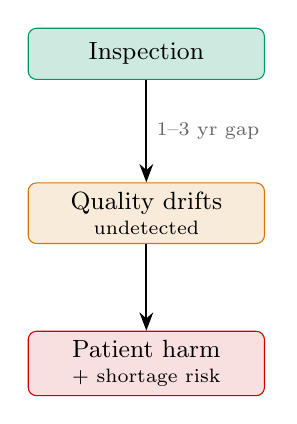
\begin{tikzpicture}[
  box/.style={rectangle, rounded corners=3pt, draw, minimum width=3.0cm,
              minimum height=0.65cm, font=\small, align=center},
  arr/.style={-{Stealth}, thick}
]
\node[box, fill=govGreen!20, draw=govGreen] (insp) {Inspection};
\node[box, fill=warnOrange!15, draw=warnOrange, below=1.3cm of insp] (drift)
  {Quality drifts\\[-2pt]{\scriptsize undetected}};
\node[box, fill=ncsuRed!12, draw=ncsuRed, below=1.1cm of drift] (harm)
  {Patient harm\\[-2pt]{\scriptsize + shortage risk}};
\draw[arr] (insp) -- node[right, font=\scriptsize, text=ncsuGray] {1--3 yr gap} (drift);
\draw[arr] (drift) -- (harm);
\end{tikzpicture}
\end{columns}
\end{frame}

\begin{frame}{FDA Form 483: Structure and the Classification Gap}
\begin{columns}[T]
\column{0.40\textwidth}

{\small \textbf{After each FDA facility inspection:}}

\vspace{6pt}
{\small
\textbf{Day of close:} \textbf{Form 483} issued \textit{if violations found} -- inspector-written list of deficiencies\\[5pt]
\textbf{Back at office:} \textbf{EIR} (Establishment Inspection Report) -- full narrative, exhibits, company responses\\[5pt]
\textbf{Later:} FDA assigns final classification\\[4pt]
\quad \textcolor{govGreen}{\textbf{NAI}} ~\textcolor{ncsuGray}{\small No Action}\\
\quad \textcolor{warnOrange}{\textbf{VAI}} ~\textcolor{ncsuGray}{\small Voluntary Action}\\
\quad \textcolor{ncsuRed}{\textbf{OAI}} ~\textcolor{ncsuGray}{\small Official Action}
}

\vspace{8pt}
\begin{itemize}
  \setlength{\itemsep}{6pt}
  \item<2-> We have \textbf{483 text} (via Redica/FOIA) -- EIR not yet accessible
  \item<3-> Relying on three labels alone \textbf{discards} most of what the inspection produced -- 483 text carries what the label does not
\end{itemize}

\column{0.57\textwidth}
\begin{center}
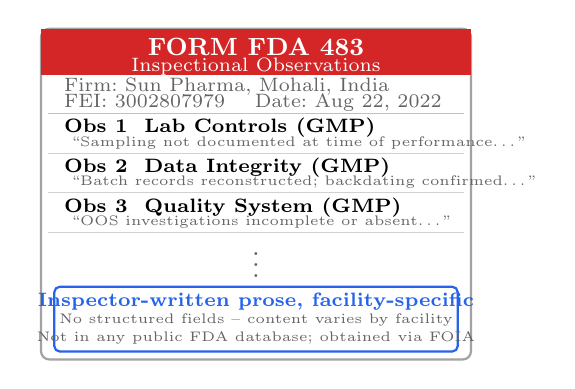
\begin{tikzpicture}[scale=0.84]
\draw[rounded corners=3pt, thick, draw=ncsuGray!60, fill=white]
  (0,0) rectangle (6.5,5.0);
\fill[ncsuRed!85] (0,4.3) rectangle (6.5,5.0);
\node[white, font=\small\bfseries] at (3.25,4.72) {FORM FDA 483};
\node[white, font=\scriptsize] at (3.25,4.43) {Inspectional Observations};
\node[right, font=\scriptsize, text=ncsuGray] at (0.2,4.12)
  {Firm:~Sun Pharma, Mohali, India};
\node[right, font=\scriptsize, text=ncsuGray] at (0.2,3.88)
  {FEI:~3002807979 \quad Date:~Aug 22, 2022};
\draw[ncsuGray!40] (0.1,3.72) -- (6.4,3.72);
\node[right, font=\scriptsize\bfseries] at (0.2,3.50)
  {Obs 1~~Lab Controls (GMP)};
\node[right, font=\tiny, text=ncsuGray] at (0.3,3.28)
  {``Sampling not documented at time of performance\ldots''};
\draw[ncsuGray!30] (0.1,3.12) -- (6.4,3.12);
\node[right, font=\scriptsize\bfseries] at (0.2,2.90)
  {Obs 2~~Data Integrity (GMP)};
\node[right, font=\tiny, text=ncsuGray] at (0.3,2.68)
  {``Batch records reconstructed; backdating confirmed\ldots''};
\draw[ncsuGray!30] (0.1,2.52) -- (6.4,2.52);
\node[right, font=\scriptsize\bfseries] at (0.2,2.30)
  {Obs 3~~Quality System (GMP)};
\node[right, font=\tiny, text=ncsuGray] at (0.3,2.08)
  {``OOS investigations incomplete or absent\ldots''};
\draw[ncsuGray!30] (0.1,1.92) -- (6.4,1.92);
\node[font=\normalsize, text=ncsuGray] at (3.25,1.55) {\vdots};
\draw[techBlue, rounded corners=2pt, thick] (0.2,0.12) rectangle (6.3,1.1);
\node[font=\scriptsize\bfseries, text=techBlue] at (3.25,0.88)
  {Inspector-written prose, facility-specific};
\node[font=\tiny, text=ncsuGray] at (3.25,0.60)
  {No structured fields -- content varies by facility};
\node[font=\tiny, text=ncsuGray] at (3.25,0.32)
  {Not in any public FDA database; obtained via FOIA};
\end{tikzpicture}
\end{center}

\vspace{4pt}
\onslide<4->{
\begin{alertblock}{Research question}
\small Do 483 text signals predict patient harm and differentiate facilities with the same outcome label?
\end{alertblock}
}
\end{columns}
\end{frame}

% ── SECTION 2: STUDY DESIGN ──────────────────────────────────────────────────
\section{Study Design \& Data}

\begin{frame}{Study Design: 14 Drugs, 98 Facilities, 2018–2026}

\onslide<1->{
\textbf{Drug and facility universe:}
\begin{itemize}
  \item \highlight{14 generic APIs} spanning cardiovascular, anti-infective, and critical care classes
  \item 129 facilities (FEIs) identified by tracing NDC codes through DailyMed product labels to manufacturer and facility identifiers
\end{itemize}
}

\vspace{5pt}
\onslide<2->{
\textbf{Inspection text and outcomes (Redica):}
\begin{itemize}
  \item \highlight{98 FEIs} with Form 483 text and NAI/VAI/OAI classifications
  \item \highlight{246 inspection events}, 2018--2026
\end{itemize}
}

\vspace{5pt}
\onslide<3->{
\textbf{Outcome variable: serious adverse events (FAERS):}
\begin{itemize}
  \item Each FAERS report carries an ANDA number -- linked to the producing facility via Orange Book crosswalk
  \item Restricted to serious outcomes: death, hospitalization, life-threatening, disability
  \item \highlight{78 of 98 FEIs} have ANDA-matched AE data; 20 have no FAERS reports citing their ANDA
\end{itemize}
}

\vspace{5pt}
\onslide<4->{
\textbf{Panel:} one row per inspection, $\pm$4 quarters. \highlight{246 rows} total (text features); \highlight{176 rows} with ANDA-matched outcome.
}

\end{frame}

% ── SECTION 3: LLM PIPELINE ──────────────────────────────────────────────────
\section{LLM Extraction Pipeline}

\begin{frame}{Pipeline: From 483 Text to Structured Features}

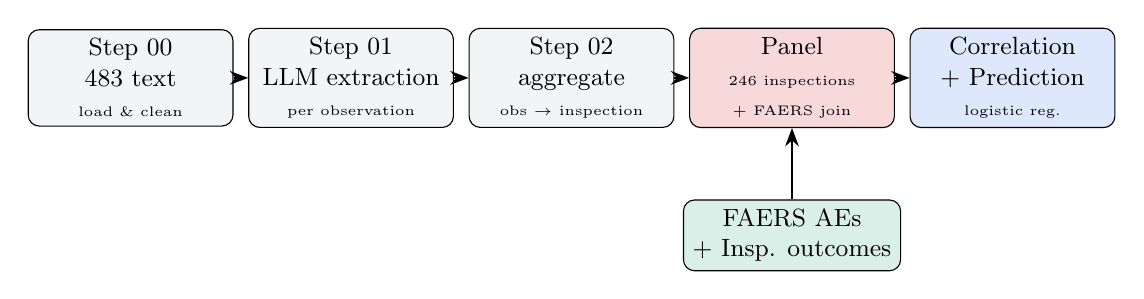
\begin{tikzpicture}[
  box/.style={rectangle, rounded corners=4pt, draw, fill=lightGray,
              minimum height=0.7cm, minimum width=2.6cm, font=\small, align=center},
  arrow/.style={-{Stealth}, thick}
]
% Step 0
\node[box] (s0) at (0,0) {Step 00\\483 text\\{\tiny load \& clean}};
% Step 1
\node[box] (s1) at (2.8,0) {Step 01\\LLM extraction\\{\tiny per observation}};
% Step 2
\node[box] (s2) at (5.6,0) {Step 02\\aggregate\\{\tiny obs $\to$ inspection}};
% Panel
\node[box, fill=ncsuRed!15] (panel) at (8.4,0) {Panel\\{\tiny 246 inspections}\\{\tiny + FAERS join}};
% Model
\node[box, fill=techBlue!15] (model) at (11.2,0) {Correlation\\+ Prediction\\{\tiny logistic reg.}};

\draw[arrow] (s0) -- (s1);
\draw[arrow] (s1) -- (s2);
\draw[arrow] (s2) -- (panel);
\draw[arrow] (panel) -- (model);

% Data joins below panel
\node[box, fill=govGreen!15] (faers) at (8.4,-2.0) {FAERS AEs\\+ Insp. outcomes};
\draw[arrow] (faers) -- (panel);

\end{tikzpicture}

\end{frame}

% ── SECTION 4: LLM EXTRACTION ────────────────────────────────────────────────
\section{LLM Extraction Pipeline}

\begin{frame}{Step 00: What a 483 Observation Looks Like in Practice}
{\small \textbf{Sun Pharma, Mohali -- Aug 2022 OAI inspection.} 6 observations. Two shown below.}

\vspace{5pt}
\begin{columns}[T]
\column{0.48\textwidth}
\onslide<1->{
\begin{block}{Observation 1 \hfill \textcolor{warnOrange}{\scriptsize Data Integrity}}
\scriptsize
\textbf{Header:} ``There is a failure to thoroughly review any unexplained discrepancy whether or not the batch has been already distributed.''

\vspace{4pt}
\textbf{Sub-item:} ``Disclosure 2020-01 confirmed instances of backdating by QA and QC personnel. The investigation was not thorough to evaluate the scope of backdating in the QA and QC departments.''

\vspace{3pt}
\textit{[3 sub-items with nested detail -- 2 pages]}
\end{block}
}

\column{0.48\textwidth}
\onslide<2->{
\begin{block}{Observation 2 \hfill \textcolor{techBlue}{\scriptsize Lab Controls}}
\scriptsize
\textbf{Header:} ``Established sampling plans, test procedures and laboratory control mechanisms are not documented at the time of performance.''

\vspace{4pt}
\textbf{Sub-item:} ``Building access records showed an employee responsible for collecting samples did not enter the buildings where samples were documented to have been collected.''

\vspace{3pt}
\textit{[2 sub-items with dated examples -- 1.5 pages]}
\end{block}
}
\end{columns}

\vspace{6pt}
{\small
\begin{itemize}
  \setlength{\itemsep}{3pt}
  \item<3-> \textbf{One inspection, two domains} -- each with different risk implications
  \item<4-> Risk signals are embedded in prose; no structured fields -- reading is required
  \item<5-> Inspector-written and facility-specific: Jaccard similarity averages 0.10 across 1,067 observations
\end{itemize}
}
\end{frame}

\begin{frame}{Step 01: What the LLM Extracts}
\begin{columns}[T]
\column{0.50\textwidth}
\textbf{Group 1: Binary flags} {\footnotesize (True/False per observation)}

\vspace{3pt}
{\small
\begin{itemize}
  \setlength{\itemsep}{4pt}
  \item \textbf{Data integrity (DI)} -- falsification, backdating, reconstructed records
  \item \textbf{Contamination} -- microbial, chemical, or cross-contamination
  \item \textbf{Patient risk} -- observation has a direct patient harm pathway
  \item \textbf{Investigation failure} -- OOS investigation absent or inadequate
  \item \textbf{Repeat finding} -- same citation appeared at a prior inspection
\end{itemize}
}

\column{0.47\textwidth}
\pause
\textbf{Group 2: Multi-category signals}

\vspace{3pt}
{\small
\begin{itemize}
  \setlength{\itemsep}{4pt}
  \item \textbf{Domain} -- 8 CFR\,211 areas (Lab Controls, Quality System\ldots)
  \item \textbf{Severity} -- Critical / Major / Moderate / Minor
  \item \textbf{Root cause} -- Capital (resource gap) vs.\ Cultural (management gap)
  \item \textbf{Scope} -- SingleBatch / MultipleProducts / FacilityWide
  \item \textbf{Remediation} -- corrective action language present or absent
\end{itemize}
}
\end{columns}
\end{frame}

\begin{frame}{Step 01: Turning Unstructured Inspection Text into Structured Features}
\begin{columns}[T]
\column{0.58\textwidth}
\begin{block}{Input: verbatim 483 observation text}
\scriptsize
``Batch production records were not completed at the time of manufacture. Entries were reconstructed from memory 2 days after processing.''
\end{block}

\vspace{4pt}
\textbf{Output (Claude Haiku, one pass per observation):}

\vspace{2pt}
{\scriptsize
\begin{tabular}{lll}
\toprule
Dimension & Extracted value & Rationale \\
\midrule
Severity & \textbf{Major} & confirmed defect; records reconstructed \\
DI flag  & \textbf{True}  & reconstructed entries = DI trigger \\
\bottomrule
\end{tabular}
}

\vspace{8pt}
{\small
\begin{itemize}
  \setlength{\itemsep}{5pt}
  \item Fixed JSON schema prevents the model from adding or inventing fields
  \item Future work: benchmark multiple LLMs for robustness, guided by the human-in-the-loop verification Redica provides
\end{itemize}
}

\column{0.39\textwidth}
\textbf{How trustworthy is the extraction?}

\vspace{5pt}
\begin{itemize}
  \setlength{\itemsep}{5pt}
  \item LLMs achieve 90\%+ accuracy on structured extraction from clinical documents; Claude 3.0 Haiku reaches 90.2\% on clinical entity extraction (Khairallah et al., 2024)
  \item Prompt definitions reviewed by Redica GMP specialists (June 2026) -- key dimensions align with industry practice
  \item Ground-truth human labeling is in progress; findings should be treated as preliminary
\end{itemize}
\end{columns}
\end{frame}

\begin{frame}{Step 02: From Observation Labels to Inspection Feature Vectors}
\begin{columns}[T]
\column{0.52\textwidth}
\textbf{Three types of features per inspection:}

\vspace{6pt}
\textbf{1. Share} -- fraction of observations in a domain or with a flag\\
{\small\textit{e.g.} \texttt{vc\_labcontrols\_share}: what kind of inspection was this?}

\pause
\vspace{6pt}
\textbf{2. Count} -- raw number of observations in a domain\\
{\small\textit{e.g.} \texttt{n\_labcontrols\_obs}: how much was cited?}

\pause
\vspace{6pt}
\textbf{3. Co-occurrence} -- both signals present in the same inspection\\
{\small\textit{e.g.} \texttt{joint\_labctrl\_di}: Lab Controls \emph{and} DI in one visit}

\column{0.45\textwidth}
\textbf{Why co-occurrence matters:}

\vspace{6pt}
{\small
Lab Controls alone: a QC process failed.\\[4pt]
DI alone: a record was altered.\\[4pt]
\textbf{Both together:} QC failures and documentation manipulation in the same inspection -- a stronger combined signal than either alone.
}

\vspace{10pt}
\begin{block}{Output}
\small 246 inspections $\times$ 17 features
\end{block}
\end{columns}
\end{frame}

% ── SECTION 5: THEORY ────────────────────────────────────────────────────────
\section{Analysis}

\begin{frame}
\begin{center}
\vspace{2.2cm}
{\Large \textbf{Analysis \& Results}}\\[14pt]
{\normalsize Are 483 text signals associated with future patient harm?\\[6pt]
Among VAI facilities -- where FDA's label provides no differentiation --\\does text separate high- from low-harm producers?}
\end{center}
\end{frame}

\begin{frame}{483 Text Signals: Two Snapshots, Two Different Stories}
\begin{columns}[T]
\column{0.56\textwidth}
\textbf{Spearman $\rho$ six months before (Q-2) and six months after (Q+2) inspection, manufacturer-specific AEs:}

\vspace{4pt}
{\small
\begin{tabular}{lcclc}
\toprule
Feature & $\rho_{\text{Q-2}}$ & & $\rho_{\text{Q+2}}$ & \\
\midrule
\texttt{severity\_critmajor}    & \tech{+0.16} & *   & \tech{+0.29} & *** \\
\texttt{n\_labcontrols\_obs}    & +0.13 &     & \tech{+0.18} & *   \\
\texttt{vc\_labcontrols\_share} & +0.09 &     & +0.13        &     \\
\texttt{data\_integrity\_flag}  & +0.06 &     & +0.09        &     \\
\midrule
\texttt{cultural\_root\_cause}  & $-$0.06 &   & $-$0.12      &     \\
\bottomrule
\multicolumn{5}{l}{\scriptsize * $p{<}.05$\quad ** $p{<}.01$\quad *** $p{<}.001$ \quad Full heatmap: backup slide}
\end{tabular}
}

\hfill\column{0.38\textwidth}
\begin{itemize}
  \setlength{\itemsep}{8pt}
  \item \textbf{Q-2:} severity already significant -- more severe findings, more AEs before FDA arrived
  \item \textbf{Q+2:} Lab Controls joins; severity strengthens further
  \item Severity captures current harm; Lab Controls predicts what follows
\end{itemize}

\end{columns}
\end{frame}

% ── SECTION 6: PREDICTIVE MODEL ──────────────────────────────────────────────
\section{Predictive Model}

\begin{frame}{From Correlation to Prediction: The VAI-Only Test}
\begin{columns}[T]
\column{0.50\textwidth}
\textbf{Why VAI-only facilities are the critical test:}

\vspace{6pt}
\begin{itemize}
  \setlength{\itemsep}{8pt}
  \item 73 facilities in our sample were \emph{never} classified OAI -- every inspection ended as VAI or NAI
  \item Within this group the outcome label never varies -- 483 text is the only available signal to differentiate facilities
\end{itemize}

\vspace{10pt}
\begin{alertblock}{Key question}
\small Does 483 text separate high- from low-harm producers where FDA's classification cannot?
\end{alertblock}

\column{0.47\textwidth}
\textbf{Prediction setup:}

\vspace{4pt}
{\small
\begin{itemize}
  \setlength{\itemsep}{5pt}
  \item \textbf{Unit:} one inspection event
  \item \textbf{Features:} 17 LLM text signals from the 483
  \item \textbf{Outcome:} above-median AEs in the post-inspection year
        $$\mathbf{1}\!\left[\,\textstyle\sum_{q=1}^{4}\,\text{AE}_{t+q} > \text{median}\,\right]$$
  \item \textbf{CV:} FEI-grouped 5-fold
  \item \textbf{Model:} logistic regression
  \item \textbf{Baseline:} AUC\,=\,0.5 (50/50 outcome by construction)
\end{itemize}
}
\end{columns}
\end{frame}

\begin{frame}{Do 483 Text Signals Carry Information? Evidence From the VAI-Only Subgroup}
\begin{columns}[T]
\column{0.50\textwidth}
\textbf{AUC, 5-fold FEI-grouped CV (176 inspections, 78 FEIs with ANDA-matched AEs):}

\vspace{4pt}
{\small
\begin{tabular}{clcc}
\toprule
 & Feature set & LR AUC & \\
\midrule
A & Text only (17 LLM features) & 0.585 & \\
B & Text + inspection outcome flag & 0.583 & \\
C & Inspection outcome flag only & 0.545 & \\
\midrule
\multicolumn{2}{l}{\textit{Random baseline}} & \textit{0.500} & \\
\midrule
\pause
\highlight{D} & \highlight{Text only, VAI-only facilities} & \highlight{0.656} & $p{=}0.046$ \\
E & Text only, OAI-ever facilities & 0.473 & \\
\bottomrule
\multicolumn{4}{l}{\scriptsize $p$ from one-tailed $t$-test vs.\ 0.5 across 5 CV folds}
\end{tabular}
}

\vspace{4pt}
{\small Config D: 55 VAI-only FEIs, 110 inspections.}

\column{0.47\textwidth}
\begin{itemize}
  \setlength{\itemsep}{7pt}
  \item \textbf{Full sample (A--C):} text (0.585) modestly outperforms the inspection outcome flag (0.545); adding the flag provides no gain
  \pause
  \item \textbf{VAI-only (D):} text reaches \highlight{AUC\,=\,0.66} ($p{=}0.046$) -- stronger signal in the subgroup where the outcome label provides no differentiation
  \pause
  \item \textbf{OAI-ever (E):} text adds little -- enforcement may have corrected the underlying problems
\end{itemize}

\vspace{8pt}
{\footnotesize \textit{Text features only -- no volume or market controls. Goal: isolate the unique contribution of 483 inspection text.}}
\end{columns}
\end{frame}

% ── SECTION 8: TRAJECTORY ANALYSIS ──────────────────────────────────────────
\section{Trajectory Analysis}

\begin{frame}{The Silent Problem: Same VAI Label, Very Different Patient Outcomes}
\begin{columns}[T]
\column{0.52\textwidth}
{\small \textbf{AEs by facility group} (98 FEIs, FEI-level medians):}

\vspace{4pt}
{\scriptsize
\begin{tabular}{lccc}
\toprule
Group & $n$ & Q0 & Q+4 \\
\midrule
OAI-ever & 25 & 32 & 30 \\
\rowcolor{techBlue!12}
Hi-sig VAI & 19 & 40 & \highlight{49} \\
Lo-sig VAI & 54 & 34 & 30 \\
\bottomrule
\end{tabular}
}

\vspace{14pt}
\pause
{\small \textbf{Top Lab Controls facilities (VAI-only), by AE rise:}}

\vspace{4pt}
{\scriptsize
\begin{tabular}{lccc}
\toprule
Manufacturer / Drug & Q0 & Q+4 & Rise \\
\midrule
Lupin / Atorvastatin      & 31 & \highlight{44} & \highlight{$+$42\%} \\
Dr.\ Reddy's / Metoprolol & 80 & \highlight{97} & \highlight{$+$21\%} \\
Sun / Atorvastatin        & 80 & \highlight{87} & \highlight{$+$9\%}  \\
\bottomrule
\end{tabular}
}

\vspace{3pt}
{\scriptsize AEs per quarter (manufacturer-specific). Hi-sig VAI = top-quartile Lab Controls share, never OAI.}

\column{0.45\textwidth}
\begin{itemize}
  \setlength{\itemsep}{9pt}
  \item Hi-sig VAI facilities produce \textbf{63\% more AEs at Q+4} than Lo-sig VAI (49 vs.\ 30), yet carry the same FDA label. Named examples show persistent AE increases with no OAI classification.
  \pause
  \item \textbf{OAI$\to$VAI downgrade:} investigative reporting (ProPublica, Bloomberg) documents cases where FDA reclassified OAI inspections to VAI, often under drug shortage pressure -- downgraded facilities show worse subsequent patient outcomes.
  \pause
  \item Alternatively, observations stayed below the OAI threshold or inspections did not surface the true severity of deficiencies.
\end{itemize}
\end{columns}
\end{frame}

% ── SECTION 10: SUMMARY ──────────────────────────────────────────────────────
\section{Summary}

\begin{frame}{Summary}

\begin{enumerate}
  \setlength{\itemsep}{8pt}
  \item \textbf{Yes -- 483 text is associated with future harm, but primarily among facilities FDA never penalized.}\\
    VAI-only AUC = \highlight{0.656}; in the full sample, text (0.585) modestly outperforms the inspection outcome flag (0.545).
  \pause

  \item \textbf{Lab Controls features are the leading text signals.}\\
    Lab Controls count and severity reach $\rho$ up to 0.29 at Q+2; no other dimension is significant at both pre- and post-inspection snapshots.
  \pause

  \item \textbf{483 text carries information the inspection outcome label does not.}\\
    The outcome label (NAI/VAI/OAI) cannot differentiate VAI facilities -- 483 text from the same visit can.
  \pause

  \item \textbf{Same VAI label, very different outcomes -- and identifiable from text.}\\
    Hi-sig VAI facilities produce 63\% more AEs at Q+4 than Lo-sig VAI (49 vs.\ 30). These facilities can be ranked from 483 text alone; shortage pressure may explain why enforcement did not follow.
\end{enumerate}

\vspace{6pt}
\begin{center}
\textit{Code: \texttt{github.com/arsahebi/drug-shortage} \quad Contact: \texttt{amirreza.sahebi@gmail.com}}
\end{center}
\end{frame}

% ── SECTION 11: LIMITATIONS & NEXT STEPS ─────────────────────────────────────
\section{Limitations \& Next Steps}

\begin{frame}{Limitations}
\begin{columns}[T]
\column{0.50\textwidth}
\begin{itemize}
  \setlength{\itemsep}{6pt}
  \item \textbf{Sample size:} 98 FEIs (78 with ANDA-matched AEs), 33 OAI inspections. VAI-only results are hypothesis-generating, not confirmatory.
  \item \textbf{COVID gap:} FDA suspended most inspections in 2020--21, leaving multi-year gaps between visits; post-2022 baselines are confounded.
  \item \textbf{FAERS attribution:} when one manufacturer operates multiple facilities under the same ANDA, we cannot determine which site produced the drug in a given report.
\end{itemize}

\column{0.47\textwidth}
\begin{itemize}
  \setlength{\itemsep}{6pt}
  \item \textbf{Extraction quality:} LLM labels require human validation. Prompt definitions for some dimensions will be revised; findings should be treated as preliminary.
  \item \textbf{Volume:} commercial volume not integrated; facility size is a potential confounder.
  \item \textbf{Causal:} all associations are correlational. Testing the shortage-pressure hypothesis requires market concentration data.
\end{itemize}
\end{columns}
\end{frame}

\begin{frame}{Next Steps}
\begin{itemize}
  \setlength{\itemsep}{8pt}
  \item \textbf{Refine LLM extraction:} update prompts based on expert feedback, validate against manual human labels.
  \item \textbf{Add MarketScan as outcome source:} MarketScan links prescriptions to NDC-level dispensing records and patient outcomes -- a cleaner tie between facility and harm than FAERS.
  \item \textbf{Add volume controls:} SDUD (Medicaid utilization) has known limitations; commercial volume data would better capture facility-level market share as a confounder.
\end{itemize}
\end{frame}

% ── Q&A SLIDE ─────────────────────────────────────────────────────────────────

\begin{frame}{}
\begin{center}
\vspace{2.2cm}
{\Large \textbf{Questions \& Discussion}}\\[20pt]
{\normalsize \texttt{amirreza.sahebi@gmail.com}}\\[8pt]
{\normalsize Code: \texttt{github.com/arsahebi/drug-shortage}}
\end{center}
\end{frame}

% ── BACKUP SLIDES ─────────────────────────────────────────────────────────────
\appendix
\section*{Backup Slides}

% --- Case study ---
{\setbeamercolor{background canvas}{bg=white}
\begin{frame}{Backup: Sun Pharma Atorvastatin -- VAI Signals, Rising AEs, OAI Follow-up}
\begin{columns}[T]
\column{0.60\textwidth}
\includegraphics[width=\linewidth]{figures/fei_case_study_3002807979.png}

\column{0.37\textwidth}
\begin{itemize}\small
  \item \textbf{2018--19 (NAI):} Clean baseline, AEs $\approx$85/qtr
  \item \textbf{Feb 2020 (VAI):} LC = 100\%, Contam = 100\%. No enforcement.
  \item \textbf{2021--22:} AEs stay at 93--112/qtr. No return visit.
  \item \textbf{Aug 2022 (OAI):} FDA escalates. AEs reach 140 at Q+4.
\end{itemize}

\vspace{4pt}
\begin{block}{Takeaway}
\small Sun Pharma was VAI-only at the 2020 visit -- 483 text from that inspection was associated with elevated AEs the following year. OAI followed in 2022.
\end{block}
\end{columns}
\end{frame}
}

% --- Study design: FAERS attribution ---
\begin{frame}{Backup: FAERS Attribution -- Design Rationale}
\begin{columns}[T]
\column{0.50\textwidth}
\textbf{Why Primary Suspect only?}\\[4pt]
FAERS reports list all drugs a patient was taking. Only the PS was judged by the reporter to have caused the event. Including concomitant or interacting drugs would attribute AEs to bystander medications and inflate counts at every facility.

\vspace{8pt}
\textbf{Why first-word drug name match?}\\[4pt]
``Atorvastatin Calcium'' in \texttt{prod\_ai} has two words. Any-word matching recovers a handful of missed combination products but mis-attributes ``Calcium'' rows to Calcium Gluconate FEIs. First-word-only is the safer tradeoff; the unmatched 0.9\% is negligible.

\column{0.47\textwidth}
\textbf{Why not a rate (AEs / volume)?}\\[4pt]
SDUD Medicaid volume covers only 69\% of FEI-years. Dividing by a partially missing denominator introduces systematic bias -- facilities with missing SDUD look artificially high-risk. AE count enters as the raw outcome; $\log(\text{SDUD units})$ enters as a covariate when available.

\vspace{8pt}
\textbf{Why serious outcomes only?}\\[4pt]
Non-serious reports are subject to much higher underreporting variability. Serious AEs have mandatory reporting paths (MedWatch, expedited), making the count more comparable across facilities and time periods.
\end{columns}
\end{frame}

% --- LLM extraction: dimensions ---
{\setbeamercolor{background canvas}{bg=white}
\begin{frame}{Backup: Observation-Level Dimensions (1 of 2)}
{\scriptsize\setlength{\tabcolsep}{4pt}
\begin{tabular}{p{1.5cm} p{3.8cm} p{3.8cm}}
\toprule
\textbf{Signal} & \textbf{What it captures} & \textbf{Why extracted} \\
\midrule
Domain & Which of 8 CFR\,211 areas: Lab Controls, Quality System, Production, Buildings \& Equipment, Materials, Records, Packaging, Personnel & Different domains carry different patient risk; Lab Controls most directly linked to product failures \\[3pt]
Severity & Confirmed defect (Major/Critical) vs.\ systemic risk without confirmed product impact & Separates inspections where defective product was likely already distributed \\[3pt]
Data integrity & Falsification, backdating, deleted or reconstructed documentation & Intentional concealment; among the most serious CGMP violations \\[3pt]
Contamination & Microbial, chemical, or cross-contamination of product or environment & Direct patient harm pathway; distinct from documentation failures \\[3pt]
Patient risk & Failure mode with a plausible patient harm pathway & Filters high-consequence citations from routine procedural ones \\
\bottomrule
\end{tabular}
}
\end{frame}
}

{\setbeamercolor{background canvas}{bg=white}
\begin{frame}{Backup: Observation-Level Dimensions (2 of 2)}
{\scriptsize\setlength{\tabcolsep}{4pt}
\begin{tabular}{p{1.5cm} p{3.8cm} p{3.8cm}}
\toprule
\textbf{Signal} & \textbf{What it captures} & \textbf{Why extracted} \\
\midrule
Investigation failure & OOS investigation absent or inadequate & Systemic gap linked to potential distribution of non-conforming product \\[3pt]
Repeat finding & Same citation appeared at a prior inspection & Facility has not corrected a known problem \\[3pt]
Scope & SingleBatch / MultipleProducts / FacilityWide & Broader scope = more patients potentially exposed \\[3pt]
Root cause & Capital (resource gap) vs.\ Cultural (management gap) vs.\ Mixed & Cultural gaps harder to fix; associated with worse future trajectories \\[3pt]
Remediation & Corrective action language present or absent & Absence expected in 483s; presence signals inspector emphasis \\
\bottomrule
\end{tabular}
}
\end{frame}
}

% --- All 17 features ---
\begin{frame}{Backup: All 17 Inspection-Level Features}
\begin{columns}[T]
\column{0.50\textwidth}
{\scriptsize
\textbf{Share features} {\tiny(fraction of observations per inspection)}
\begin{itemize}
  \setlength{\itemsep}{1pt}
  \item \texttt{vc\_labcontrols\_share} -- Lab Controls
  \item \texttt{vc\_qualitysystem\_share} -- Quality System
  \item \texttt{severity\_critmajor\_share} -- Critical/Major
  \item \texttt{contamination\_llm\_share} -- Contamination
  \item \texttt{data\_integrity\_llm\_share} -- Data integrity
  \item \texttt{patient\_risk\_llm\_share} -- Patient risk
  \item \texttt{investigation\_llm\_share} -- Investigation failure
  \item \texttt{repeat\_cross\_insp\_share} -- Repeat finding
  \item \texttt{scope\_facilitywide\_share} -- Facility-wide scope
  \item \texttt{cultural\_root\_cause\_share} -- Cultural root cause
\end{itemize}
}

\column{0.47\textwidth}
{\scriptsize
\textbf{Count features} {\tiny(raw observation count)}
\begin{itemize}
  \setlength{\itemsep}{1pt}
  \item \texttt{n\_labcontrols\_obs} -- Lab Controls
  \item \texttt{n\_qualitysystem\_obs} -- Quality System
\end{itemize}

\vspace{6pt}
\textbf{Co-occurrence flags} {\tiny(1 if both signals present in same inspection)}
\begin{itemize}
  \setlength{\itemsep}{1pt}
  \item \texttt{joint\_labcontrols\_dataintegrity}
  \item \texttt{joint\_contamination\_labcontrols}
  \item \texttt{joint\_labcontrols\_qualitysystem}
  \item \texttt{joint\_qualitysystem\_production}
  \item \texttt{multi\_domain\_insp}
\end{itemize}
}
\end{columns}
\end{frame}

% --- Correlation heatmap ---
\begin{frame}{Backup: Correlation Heatmap -- All Features, All Lags}
\begin{center}
\includegraphics[width=0.86\textwidth]{figures/lag_heatmap.png}
\end{center}
\vspace{-6pt}
{\scriptsize Full Q0--Q+4 range shown (main slides use Q-2/Q+2 snapshots). Lab Controls cluster grows from Q0 to Q+4; severity is significant across all lags; data integrity is flat. ANDA-specific AEs, $n=148$.}
\end{frame}

% --- Inspection gap distribution ---
\begin{frame}{Backup: Inspection Gap Distribution}
\begin{columns}[T]
\column{0.50\textwidth}
\textbf{All drug facilities (23,604 FEIs, 27,431 gap pairs):}
\vspace{4pt}
\begin{tabular}{lc}
\toprule
Percentile & Gap (years) \\
\midrule
P10 & 0.16 \\
P25 & 1.01 \\
P50 (median) & 2.11 \\
P75 & 3.70 \\
P90 & 5.81 \\
P95 & 7.17 \\
Max & 16.26 \\
\bottomrule
\end{tabular}

\vspace{6pt}
Gaps $>$ 3yr: 33.3\% of pairs\\
Gaps $>$ 2yr: 52.7\% of pairs\\
Gaps $<$ 1yr: 24.6\% of pairs

\column{0.47\textwidth}
\textbf{By previous inspection classification (our 98 FEIs):}
\vspace{4pt}
\begin{tabular}{lccc}
\toprule
Prev. class & Mean gap & Median gap & $n$ \\
\midrule
NAI & 1.78yr & 1.44yr & 193 \\
VAI & 1.77yr & 1.55yr & 372 \\
OAI & \highlight{1.55yr} & 1.41yr & 47 \\
\bottomrule
\end{tabular}

\vspace{6pt}
OAI facilities are re-inspected slightly faster, but the difference is small ($\Delta = 0.22$ yr).

\vspace{4pt}
Post-COVID gap expansion: pre-2020 median = 1.33yr $\to$ post-2022 median = 4.04yr
\end{columns}
\end{frame}

% --- Inspection gap: AEs rise ---
\begin{frame}{Backup: AEs Rise in the Year Before FDA Arrives}
\begin{columns}[T]
\column{0.62\textwidth}
{\small \textbf{AE trajectory by gap since previous inspection} (237 inspections, manufacturer-specific AEs):}

\vspace{3pt}
{\small
\begin{tabularx}{\linewidth}{l>{\centering\arraybackslash}X>{\centering\arraybackslash}X>{\centering\arraybackslash}X>{\centering\arraybackslash}X}
\toprule
Gap & $n$ & pre\_rise & persist & mean gap \\
& & AE$_{t0}$/AE$_{t{-4}}$ & AE$_{t{+4}}$/AE$_{t0}$ & (yr) \\
\midrule
$<$1yr & 60 & 1.294 & 1.024 & 0.7 \\
\rowcolor{techBlue!15}
1--2yr & 87 & \textbf{1.367} & 0.783 & 1.5 \\
2--3.5yr & 57 & 1.151 & 1.018 & 2.6 \\
$>$3.5yr & 33 & 0.931 & 1.199 & 4.4 \\
\bottomrule
\end{tabularx}
}

\vspace{5pt}
{\small \textbf{Where does $t_{-4}$ (baseline, 1yr before inspection) fall?}\\
$<$1yr: before previous inspection -- AEs already elevated.\\
1--2yr: after previous inspection -- AEs suppressed. \textbf{Clean baseline.}\\
$>$2yr: deep in quiet window -- no enforcement anchor.}

\column{0.35\textwidth}
{\small Only the 1--2yr group has a clean baseline. The 37\% pre-inspection rise is real quality drift, not a measurement artifact.}

\vspace{6pt}
{\small Persist = 0.78 for this group: enforcement works when FDA arrives. But harm was occurring throughout the rising period.}

\vspace{6pt}
{\small AEs were already rising before FDA arrived -- the quality problem preceded the visit. The 483 text captures what inspectors found at the end of this drift.}
\end{columns}
\end{frame}

% --- Volume control ---
\begin{frame}{Backup: Volume Control -- SDUD Medicaid Utilization}
\begin{columns}[T]
\column{0.52\textwidth}
A larger manufacturer generates more FAERS reports at the same defect rate. Raw AE counts conflate facility size with quality.

\vspace{6pt}
\textbf{CMS SDUD}: all 50 states, quarterly, 2015--2024. Join: labeler + product code $\to$ DailyMed NDC-FEI crosswalk.

\vspace{6pt}
\begin{tabular}{ll}
\toprule
Metric & Value \\
\midrule
FEI-year coverage & \highlight{69\%} \\
Mean annual units/FEI & 237M \\
Median AE rate & 49 AEs / M units \\
\bottomrule
\end{tabular}

\vspace{6pt}
Use $\log(\text{sdud\_units})$ as a covariate, not a rate denominator. 31\% missing coverage biases the rate.

\column{0.45\textwidth}
\begin{tabular}{lcc}
\toprule
Group & SDUD units & AE rate \\
\midrule
Never-OAI & 239M & 19,847/M \\
Ever-OAI  & 203M & 8,925/M \\
\bottomrule
\end{tabular}

\vspace{8pt}
Rate is inverted vs.\ raw counts: a matching artifact from the 31\% gap, not a real quality signal.

\vspace{8pt}
\begin{block}{Limitation}
SDUD covers Medicaid only ($\sim$20\% of market). IQVIA commercial data needed for full volume control.
\end{block}
\end{columns}
\end{frame}

% --- Quarterly trajectory ---
\begin{frame}{Backup: Quarterly Trajectory by OAI vs VAI/NAI Classification}
\begin{columns}[T]
\column{0.55\textwidth}
\textbf{Inspection-centered panel, manufacturer-specific AEs} (176 events with ANDA-matched AEs, $\pm$4 quarters):

\vspace{4pt}
\begin{tabular}{lccc}
\toprule
Quarter & All & VAI/NAI & OAI \\
& (246) & (213) & (33) \\
\midrule
$t-4$ & 35.7 & 36 & 33 \\
$t-3$ & 36.6 & & \\
$t-2$ & 40.5 & & \\
$t-1$ & 40.7 & & \\
$t=0$ & 43.1 & 46 & 30 \\
$t+1$ & 41.7 & & \\
$t+2$ & 39.9 & & \\
$t+3$ & 44.0 & & \\
$t+4$ & 42.2 & \highlight{44} & \highlight{33} \\
\midrule
pre\_rise & & 1.258 & 0.926 \\
persist & & 0.965 & 1.073 \\
\bottomrule
\end{tabular}

\vspace{4pt}
{\scriptsize
\textbf{pre\_rise} = AE($t_0$) / AE($t_{-4}$): rise in the year before inspection.\\
\textbf{persist} = AE($t_{+4}$) / AE($t_0$): persistence in the year after.}

\column{0.42\textwidth}
\begin{enumerate}
  \item \textbf{Both groups persist.} persist $\approx$ 1.05 for both OAI and VAI/NAI. Enforcement takes more than one year to clear pre-inspection product from the market.

  \item \textbf{Pre-inspection rise differs.} VAI/NAI pre\_rise = 1.18 vs OAI 1.06. FDA escalates based on what inspectors see, not on FAERS trends.

  \item \textbf{Implication:} OAI label alone does not separate which facilities improve. This motivates using 483 text instead.
\end{enumerate}
\end{columns}
\end{frame}

% --- Trajectory clustering ---
\begin{frame}{Backup: AE Trajectory Clustering (Drug-Level)}
\begin{columns}[T]
\column{0.54\textwidth}
{\small Each facility summarized as one row (median across inspection events); \textbf{t here is years}, not quarters.}

\vspace{5pt}
{\small KMeans ($k=4$) on slope\_pre, slope\_post, persist, pre\_rise:}

\vspace{3pt}
{\small
\begin{tabular}{lcccc>{\columncolor{lightGray}}c}
\toprule
Cluster & $n$ & pre\_rise & persist & tech & OAI \\
\midrule
\highlight{Flat/rising} & 3 & \highlight{4.63} & \highlight{0.96} & 0.39 & 0\% \\
Spike-correct & 28 & 1.14 & 0.93 & \highlight{0.62} & 14\% \\
Slow-decline & 66 & 1.02 & 0.87 & 0.33 & 21\% \\
Flat-low & 2 & 1.11 & 0.30 & 0.42 & 0\% \\
\bottomrule
\end{tabular}
}

\vspace{4pt}
{\scriptsize tech = composite Lab Controls + DI score; OAI = share ever-OAI\\
pre\_rise = AE$_{t0}$/AE$_{t-2}$; persist = AE$_{t+2}$/AE$_{t0}$}

\column{0.43\textwidth}
{\small
\textbf{Flat/rising (3 FEIs):} AEs 4.6$\times$ higher at inspection than 2 years prior, keep rising after. Zero OAI ever. Silent cases the clustering identifies without any text label.

\vspace{6pt}
\textbf{Spike-correct (28):} Highest tech score (0.62), some OAI, AEs declining post-inspection. System responding.

\vspace{6pt}
\textbf{Slow-decline (66):} Majority. Gradual decline, moderate signals.

\vspace{6pt}
\textbf{Flat-low (2):} Extreme AEs collapsing 70\% post-inspection. Likely a recall, not enforcement-driven.
}
\end{columns}

\vspace{4pt}
{\scriptsize Note: drug-level AE counts (all manufacturers pooled). ANDA-specific attribution collapses most clusters; drug-level version shown for reference.}
\end{frame}

\end{document}
